\documentclass[twocolumn,aps,prc,showpacs,superscriptaddress,preprintnumbers,floatfix,nofootinbib]{revtex4}
% \documentclass[preprint,aps,prc,showpacs,superscriptaddress,preprintnumbers,floatfix,nofootinbib]{revtex4}
% \tightenlines
\usepackage{epsfig,graphics}
\usepackage{graphicx}% Include figure files
\usepackage{dcolumn}% Align table columns on decimal point
\usepackage{bm}% bold math
\usepackage{amsmath}
\usepackage[usenames]{color}
\usepackage{ulem} %% for strike-through
% \usepackage{multicol}
% \usepackage{multiraw}

\newcommand{ \auau }{$^{197}\mathrm{Au}+^{197}\mathrm{Au}$}
\newcommand{ \srt  }{$\sqrt{s_{_{\rm NN}}}$}
\newcommand{ \mpt } {$\langle p_T \rangle$}
\newcommand{ \pt } {${p_{T}}$}
\newcommand{ \Rcp } {${(R_{cp}}$}
\newcommand{ \rcp } {${R_{cp}}$}
\newcommand{\rts}   {${\sqrt{s_{NN}}}$}
\newcommand{ \p} {$\phi$}
\newcommand{\om} {$\Omega$}

\voffset=0.5in
\usepackage{CJK}
\usepackage{epstopdf}
\hfuzz=\maxdimen
\tolerance=10000
\hbadness=10000

\begin{document}
\begin{CJK*}{GBK}{song}
  \title{$\Omega$ and $\phi$ production in a multiphase transport model with enhanced local parton density fluctuation scenario}
  % \author{Y. J. Ye}
  % \affiliation{Shanghai Institute of Applied Physics, Chinese Academy of Sciences, Shanghai 201800, China}
  % \affiliation{University of Chinese Academy of Sciences, Beijing 100049, China}
  % \author{J. H. Chen}
  % \email{chenjinhui@sinap.ac.cn}
  % \affiliation{Shanghai Institute of Applied Physics, Chinese Academy of Sciences, Shanghai 201800, China}
  % \author{Y. G. Ma}
  % \email{ygma@sinap.ac.cn}
  % \affiliation{Shanghai Institute of Applied Physics, Chinese Academy of Sciences, Shanghai 201800, China}
  % \affiliation{ShanghaiTech University, Shanghai 200031, China}
  % \author{S. Zhang}
  % \affiliation{Shanghai Institute of Applied Physics, Chinese Academy of Sciences, Shanghai 201800, China}
  % \author{C. Zhong}
  % \affiliation{Shanghai Institute of Applied Physics, Chinese Academy of Sciences, Shanghai 201800, China}

  \date{\today}

  \begin{abstract}
    Searching for QCD critical point and mapping the QCD phase diagram are major science
    goals of the Beam Energy Scan program in Heavy-Ion Collisions. Multi-strange hadron
    such as $\Omega$ and $\phi$ are important probes for the search of the QCD phase
    boundaries. The $\Omega$ and $\phi$ are expected to have relatively small hadronic
    interaction cross sections. Therefore, they can carry the information directly from the
    chemical freeze-out stage with little or no distortion due to hadronic rescattering. As a
    result, the production of the $\Omega$ and $\phi$ particle offers a unique advantage in
    probing the transition from partonic to hadronic dynamics. In this paper, we study the
    $\Omega$ and $\phi$ production in a multiphase transport model with employment enhanced
    local parton density fluctuation scenario. We find that the Baryon/Meson ratio is
    sensitive to the local density fluctuation strength. We also study the flow harmonic of
    Multi-strange hadron in response to the local density fluctuation.
  \end{abstract}

  % \pacs{ 25.70.-q, 25.75.Nq}

  \maketitle
  \textbf{Keywords: multi-strangness particles, AMPT, RHIC}



  % \begin{multicols}{2}
  \section{Introduction}

  Lattice quantum chromodynamics(QCD) calculations suggest that at high temperature and
  low baryon chemical potential($\mu_{B}$), there will be a phase transition from the
  hadron gas to the quark gluon plasma(QGP), and the phase transition is smooth and
  continuous. Heavy ion collisions at relativistic energy provide a possibility to
  study the properties of QGP and QCD phase diagram. The production of multi-strange
  particles provides a way to investigate the properties of QCD phase diagram.


  \section{The ampt model}

  A multiphase transport (AMPT) model is a hybrid model to describe heavy ions
  collisions at relativistic energies~\cite{AMPT1,AMPT2,AMPT3,AMPT4}. It has two
  versions: default version and string melting version. In our study, we adopt the
  string melting version to study QCD fluctuation. Because, in string melting version,
  all the excited strings are converted into partons, it has a clear advantage
  over the default version in describing the anisotropic flows~\cite{FLOW1}.
  The AMPT model consists of four components. The initial stage is described by heavy
  ion jet interaction generator (HIJING) model~\cite{HIJING1,HIJING2} that is designed to
  simulate multiple jets and particle production in heavy ion collisions. Zhang's
  parton cascade (ZPC)~\cite{ZPC} is used to describe scattering among partons,
  until now, it only includes two-body interaction, but we think it is enough to
  describe interaction between partons. The hadronization of parton is based on a
  simple quark coalescence model~\cite{AMPT3}. The scattering of resulting hadrons is
  described by a relativistic transport (ART) model~\cite{ART1,ART2}.
  \par
  In the transport approach, interactions among partons are described by
  equations of their Wigner distribution functions, which describe semicalssically
  their density distribution in phase space. In AMPT model, the total cross section
  of parton can be described use the following equation~\cite{ZPC}
  \begin{gather}
    \label{eq:equationcrosssection}
    \frac{d\sigma_{p}}{dt} \simeq \frac{9\pi\alpha_{s}^{2}}{2(t-\mu^{2})^{2}},\\
    \sigma_{p} \simeq \frac{9\pi\alpha_{s}^{2}}{2\mu^{2}}\frac{1}{1+\mu^{2}/s}.
  \end{gather}
  where $\alpha_{s}$ is the strong coupling constant and can be a value of 0.47,
  $\mu$ is the screening mass which depend on the medium effect~\cite{ZPC},
  s and t are the usual Mandelstam variables. Using parton scattering cross sections
  of 6-10 mb, the AMPT model can reproduce the centrality and transverse momentum
  dependence of hadron elliptic flow~\cite{CROSSSECTION}. For our study, we take the
  parton scattering cross section as 10 mb~\cite{TENMB}. Until now, for the AMPT program that
  is being used, it does not contain QCD fluctuation. However, according to the
  calculation of lattice QCD, the phase transition is smooth and continuous between
  hadron gas and QGP, this implies that there may be a critical point at the
  end of the first order phase transition line. Viewed from the thermodynamic,
  a critical point is a point at which a single thermodynamic state bifurcates
  into two macroscopically distinct states. This bifurcation may leads to long-ranged
  thermal fluctuations. To model this effect, a large density fluctuation is introduced
  at the end of scattering of parton. Shown in Fig. \ref{fig:phaseSpace} is the
  distributions of parton in the transverse plane.
  \begin{figure}[htbp]
    \centering
    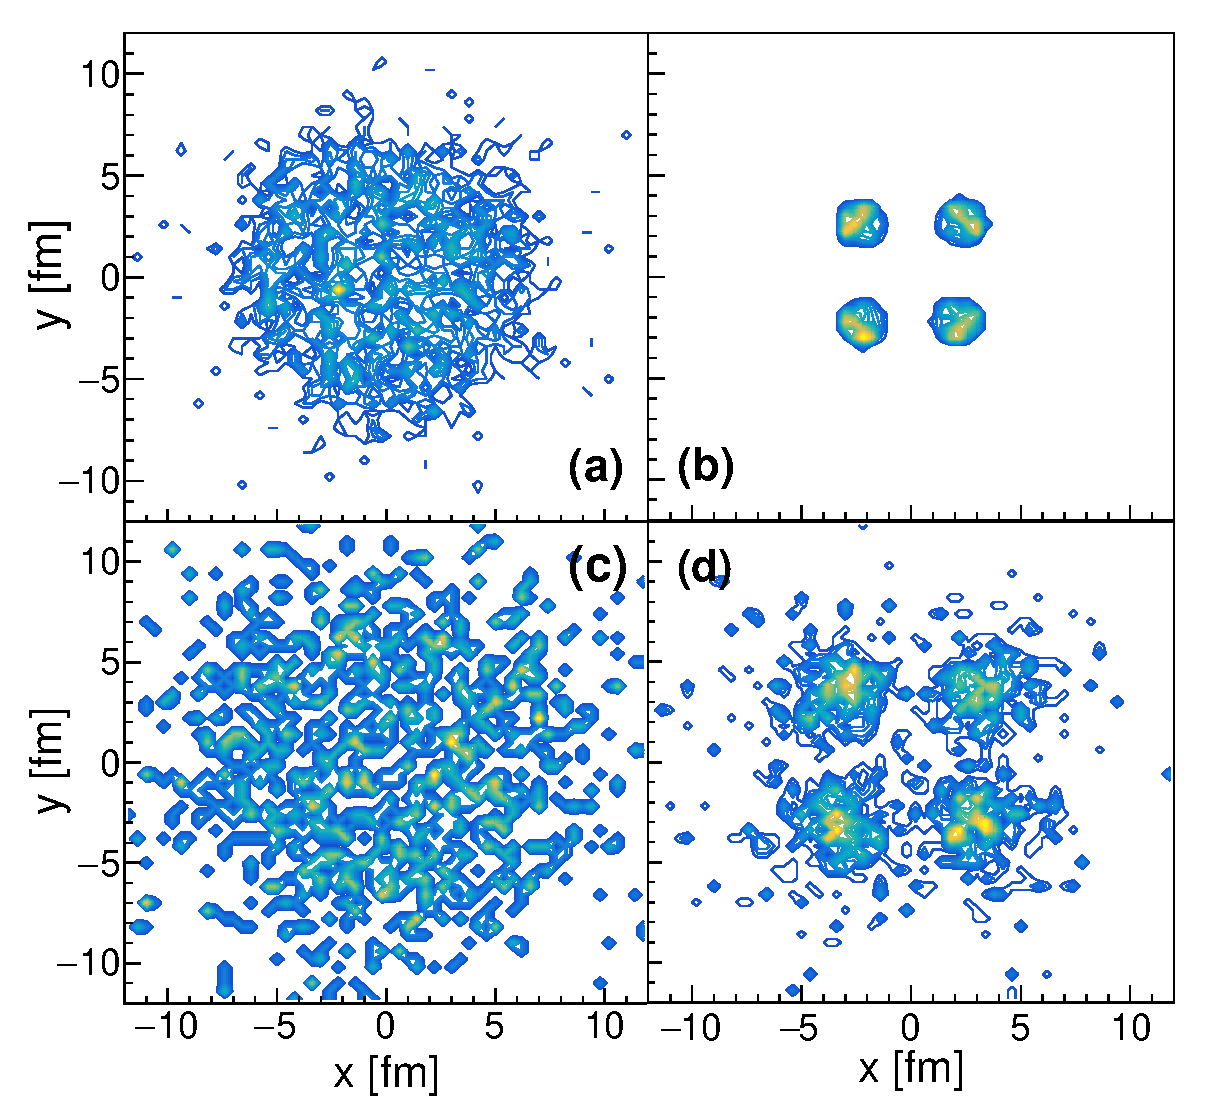
\includegraphics[width=0.45\textwidth]{./figure/square.eps}
    \caption{The distributions of parton and hadron in the transverse plane.}
    \label{fig:phaseSpace}
  \end{figure}
  The upper left is the distribution of parton without QCD fluctuation, the bottom left
  is the distribution of hadron and final-state hadronic scatterings are closed.
  Similarly, there are results about QCD fluctuation on the right. it is obvious that
  the QCD fluctuation of parton can be served in harmonic matter.


  \section{The dynamical coalescence model of $\Omega$ and $\phi$}
  A dynamical coalescence model has been used to study the production
  of $\Omega$ and $\phi$. according to this model, the probability for producing
  a hadron from partons is given by the overlap of parton phase-space distributions
  with the parton Wigner phase-space function inside hadron~\cite{COALESCENCE1}. \
  The multiplicity of a $M$-parton
  hardon in a heavy-ion collision is given by
  \begin{multline}
    \label{eq:multiplicity}
    N_{M} = G  \int{}d\bm{r}_{i_{1}}d\bm{q}_{i_{1}}\dots{}d\bm{r}_{i_{M-1}}d\bm{q}_{i_{M-1}}\\
    \times{}\langle{}\sum_{i_{1}>i_{2}>\dots>i_{M}}\rho_{i}^{W}(\bm{r}_{i_{1}},\bm{q}_{i_{1}}\dots{}\bm{r}_{i_{M-1}},\bm{q}_{i_{M-1}}) \rangle{}.
  \end{multline}
  In Eq.~(\ref{eq:multiplicity}), $\langle{}$\dots$\rangle{}$ represents the event averaging;
  $\textbf{r}_{i_{1}}$,\dots{},$\textbf{r}_{i_{M-1}}$ and
  $\textbf{q}_{i_{1}}$,\dots,$\textbf{q}_{i_{M-1}}$ are the $M-1$ relative
  coordinates and momenta in the $M$-parton rest frame; $\rho_{i}^{W}$ is the
  Wigner phase-space function inside the hadron and G is the statistical factor for
  the $M$ partons.

  To determine the quark Wigner phase-space functions inside $\Omega$ and $\phi$,
  we need quark wave functions. The quark wave functions can be token as a spherical
  harmonic oscillator~\cite{TENMB}. For the $\phi$ particle, it can be expressed as
  \begin{equation}
    \label{eq:phispherical}
    \psi(\bm{r}_{1},\,\bm{r}_{2}) = 1 / (\pi\sigma_{\phi}^{2})^{3/4}\;exp\left[-r^{2}/(2\sigma_{\phi}^{2})\right].
  \end{equation}
  where $\bm{r} = \bm{r_{1}} - \bm{r_{2}}$ is the relative coordinate and $\sigma_{\phi}$ is a size parameter
  of $\phi$, its normalized wave function
  leads to a root mean-square radius $R_{\phi} = (3/8)^{1/2}\sigma_{\phi}$. The quark
  Wigner function in $\phi$ particle can be expressed as
  \begin{equation}
    \label{eq:phiwigner}
    \rho_{\phi}^{W}(\bm{r},\bm{k}) = 8 exp\left(-\frac{r^2}{\sigma_{\phi}^2}-\sigma_{\phi}^{2}k^{2}\right).
  \end{equation}
  where \textbf{k} = ($\textbf{k}_{1}-\textbf{k}_{2})/2$ is the relative momentum
  between $s$ and $\bar{s}$.

  Similarly, for $\Omega^{-}$ and $\bar{\Omega}^{+}$ particles, their wave function
  can be described by the following equation
  \begin{equation}
    \label{eq:omegaspherical}
    \psi(\bm{r}_{1},\bm{r}_{2},\bm{r}_{3}) = (3\pi^{2}\sigma_{\Omega}^{4})^{-3/4}\,exp\left(-\frac{\rho^2+\lambda^2}{2\sigma_{\Omega}^{2}}\right).
  \end{equation}
  The quark Wigner phase-space function inside the $\Omega^{-}$ and $\bar{\Omega}^{+}$
  baryon can be expressed as
  \begin{multline}
    \label{eq:omegawigner}
    \rho_{\Omega}^{W}(\rho, \lambda, \bm{k}_{\rho}, \bm{k}_{\lambda}) = \\
    64\;exp\left(-\frac{\rho^2+\lambda^2}{\sigma_{\Omega}^{2}}\right)
    exp\left[-(\bm{k}_{\rho}^{2}+\bm{k}_{\lambda}^{2})\sigma_{\Omega}^{2}\right].
  \end{multline}
  where $\rho$ and $\lambda$ are relative coordinates of quark, $\textbf{k}_\rho$ and
  $\textbf{k}_\lambda$ are relative momenta, $\sigma_{\Omega}$ is a size parameter
  that is related to the root mean-square radius $R_{\Omega}$.

  The two parameters $\sigma_{\phi}$ and $\sigma_{\Omega}$ in the quark Wigner
  phasespace functions inside the $\phi$ meson and $\Omega$ baryon are related to
  their root-mean-square (RMS) radius. we take their values of RMS as
  $R_{\phi} = 0.65$ fm and $R_{\Omega} = 1.2$ fm~\cite{TENMB}.

  \section{Transverse momentum spectra of $\phi$ and $\Omega$}
  Using the parton phase-space information and dynamical coalescence method, we study
  the effect of QCD fluctuation on transverse-momentum spectra of $\phi$ and $\Omega$
  as well as their flow.
  \begin{figure}[htbp]
    \centering
    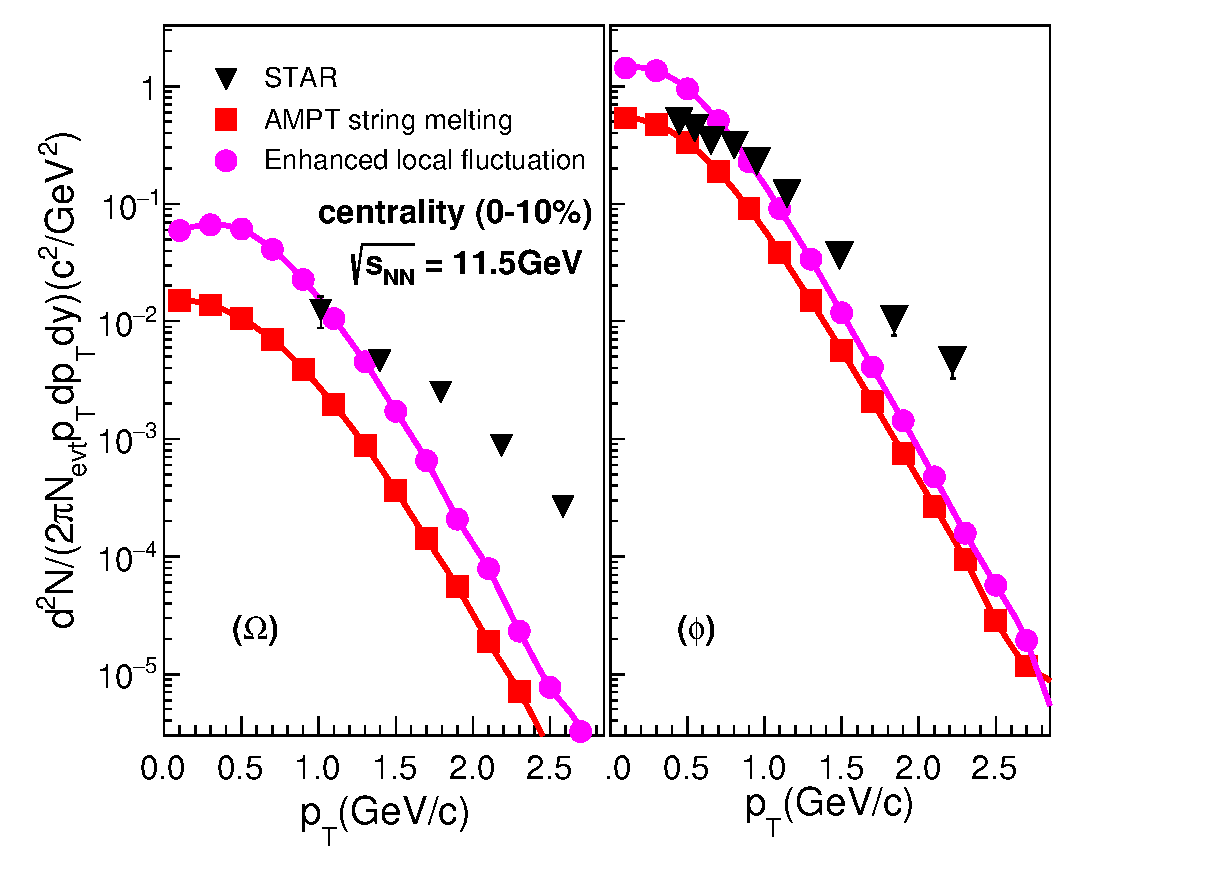
\includegraphics[width=0.45\textwidth]{./figure/yield.eps}
    \caption{The transverse momentum spectra: left panel is $\Omega$ spectra and right
      panel is $\phi$ spectra.}
    \label{fig:omegaspectra}
  \end{figure}
  In Fig. \ref{fig:omegaspectra}, we present the transverse momentum distributions
  of $\Omega$ and $\phi$ measured at midrapidity ($|y| \lesssim 1$). From these two
  figures, it is obvious that the QCD fluctuation has the trend to increase the transverse
  momentum spectra of $\Omega$ and $\phi$. As a comparison, the experimental data is
  shown~\cite{STAR}. However, in AMPT, the total number of
  strange quarks follows the same distribution in different events, in other words,
  through dynamical coalescence method, the total number of
  \textquotedblleft{strange}\textquotedblright hadron times the valence quarks number
  should satisfy the same distribution. So the transverse momentum spectra can not directly
  response the QCD fluctuation.
  \par
  Therefore, we also study the ratio of $\Omega/\phi$ as a function of $p_t$. The result
  is presented in Fig.\ref{fig:ratio},
  \begin{figure}[htpb]
    \centering
    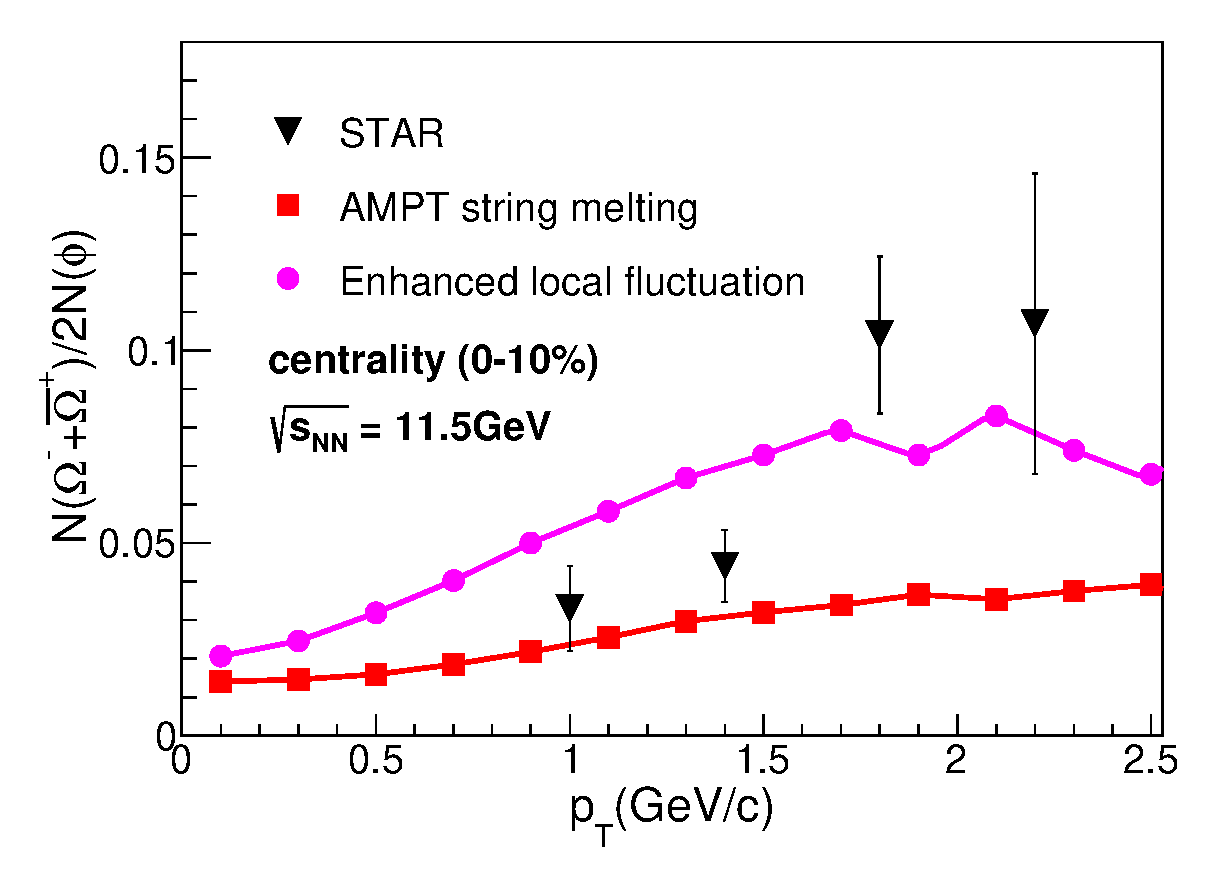
\includegraphics[width=0.45\textwidth]{./figure/ratio.eps}
    \caption{The ratio of $\Omega$ to $\phi$.}
    \label{fig:ratio}
  \end{figure}
  The measured $N(\Omega^{-}+\bar{\Omega}^{+})/2N(\phi)$ ratio from string melting
  AMPT is flat and can describe the experiment data in low $p_t$, but it underestimates
  the ratio in high $p_{t}$. For the enhanced local fluctuation result, it is obvious that
  QCD fluctuation has the trend to increase the ratio of $\Omega$ to $\phi$.

  \section{Anisotropic flows of $\phi$ and $\Omega$}
  In this section, we evaluate the effects of variations in the parton density distributions
  and discuss its effect on elliptic flow. The participant eccentricity $\varepsilon_{part}$
  can be defined as
  \begin{equation}
    \label{eq:equationeccentricity}
    \varepsilon_{part} = \frac{\sqrt{(\sigma_{y}^{2}-\sigma_{x}^{2})^2+4\sigma_{xy}^{2}}}{\sigma_{y}^{2}+\sigma_{x}^{2}}.
  \end{equation}
  where
  \begin{gather}
    \label{eq:1}
    \sigma_{x}^{2} = \{x^{2}\}-\{x\}^{2}\\
    \sigma_{y}^{2} = \{y^{2}\}-\{y\}^{2}\\
    \sigma_{xy} = \{xy\}-\{x\}\{y\},
\end{gather}
and \{\dots\} denotes the average over all participants in one event.
The result is shown in Fig.\ref{fig:figureeccentricity}. it is obvious that QCD fluctuation
does not have a greater impact on eccentricity.
\begin{figure}[hbpt]
  \centering
  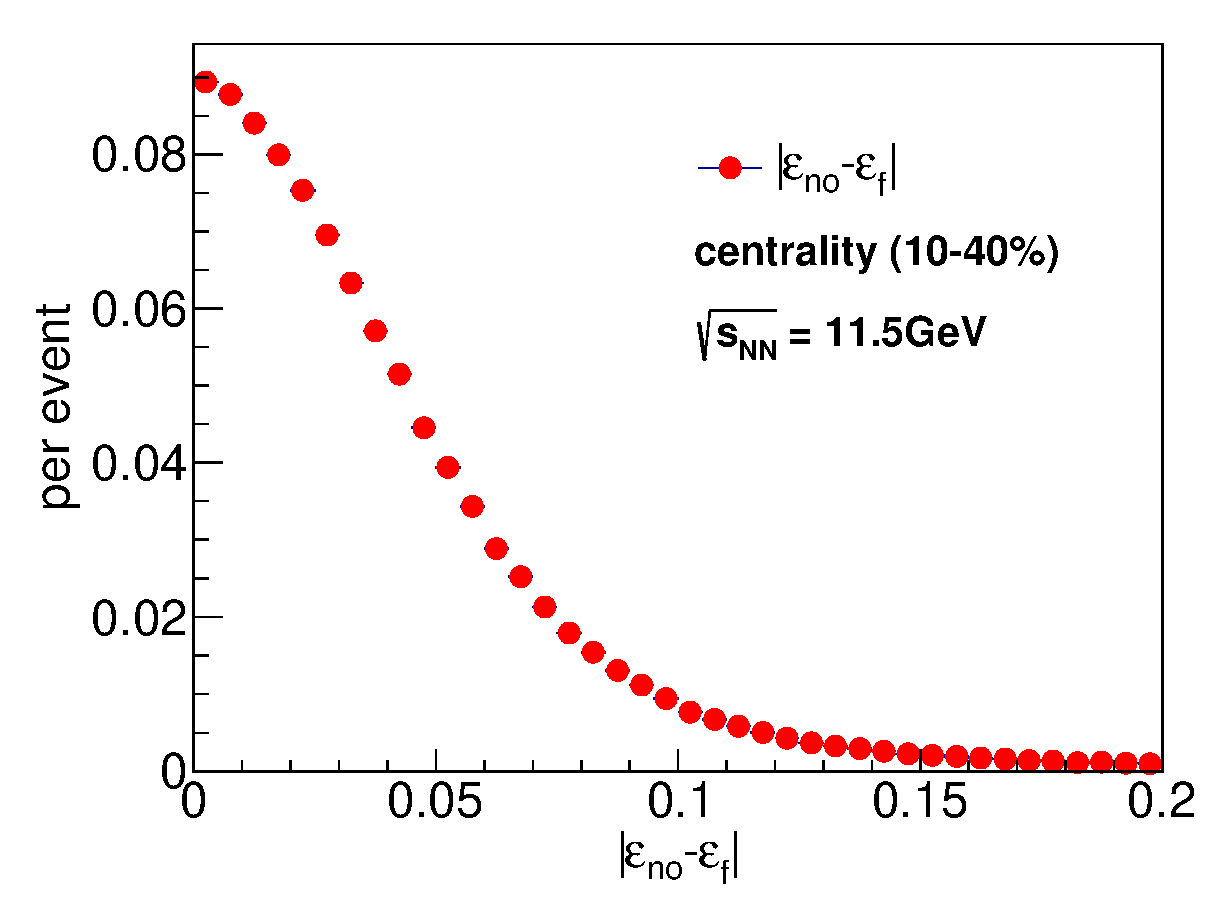
\includegraphics[width=0.45\textwidth]{./figure/eccentricity.eps}
  \caption{The result of participant eccentricity.}
  \label{fig:figureeccentricity}
\end{figure}
The collectivity in high-energy heavy-ion collisions can be measured through final particle
azimuthal anisotropy. The anisotropy coefficients are generally obtained from Fourier
expansion of final particle azimuthal distortion~\cite{MALONG}. i.e.,
\begin{equation}
  \label{eq:equationfourier}
  E\frac{d^{3}N}{d^{3}p} = \frac{1}{2\pi}\frac{d^{2}N}{p_{T}dp_{T}dy}\left(1+\sum^{N}_{i=1}{2v_{n}cos[n(\phi-\psi_{RP})]}\right).
\end{equation}
where $E$ is the energy of final particle, $p_{T}$ is the transverse momentum, y is the
rapidity, $\phi$ is the azimuthal angle of particle and $\psi_{RP}$ is the reaction plane
angle. The Fourier coefficients $v_{n}(n=1,2,\dots)$ can be described by the following equation
\begin{equation}
  \label{eq:equationflow}
  v_{n} = \langle{cos(n[\phi-\psi_{RP}])}\rangle.
\end{equation}
Similarly, the calculation of harmonic flow $v_{n}$ can be relative to the participant
plane angle $\psi_{n}\{P\}$. For the study of QCD fluctuation, we think this method is
more appropriate. The participant plane angle can be defined by the following equation
\begin{equation}
  \label{eq:equationparticipant}
  \psi_{n}\{P\} = \frac{1}{n}\left[arctan\frac{\langle{r^{2}sin(n\varphi)}\rangle}{\langle{r^{2}cos(n\varphi)}\rangle}+\pi\right].
\end{equation}
where $n$ is $n$th-order participant plane, $r$ and $\varphi$ are the coordinates position and
azimuthal angle of parton, the symbol $\langle{\dots}\rangle$ represents density weighting.
\begin{figure}[htbp]
  \centering
  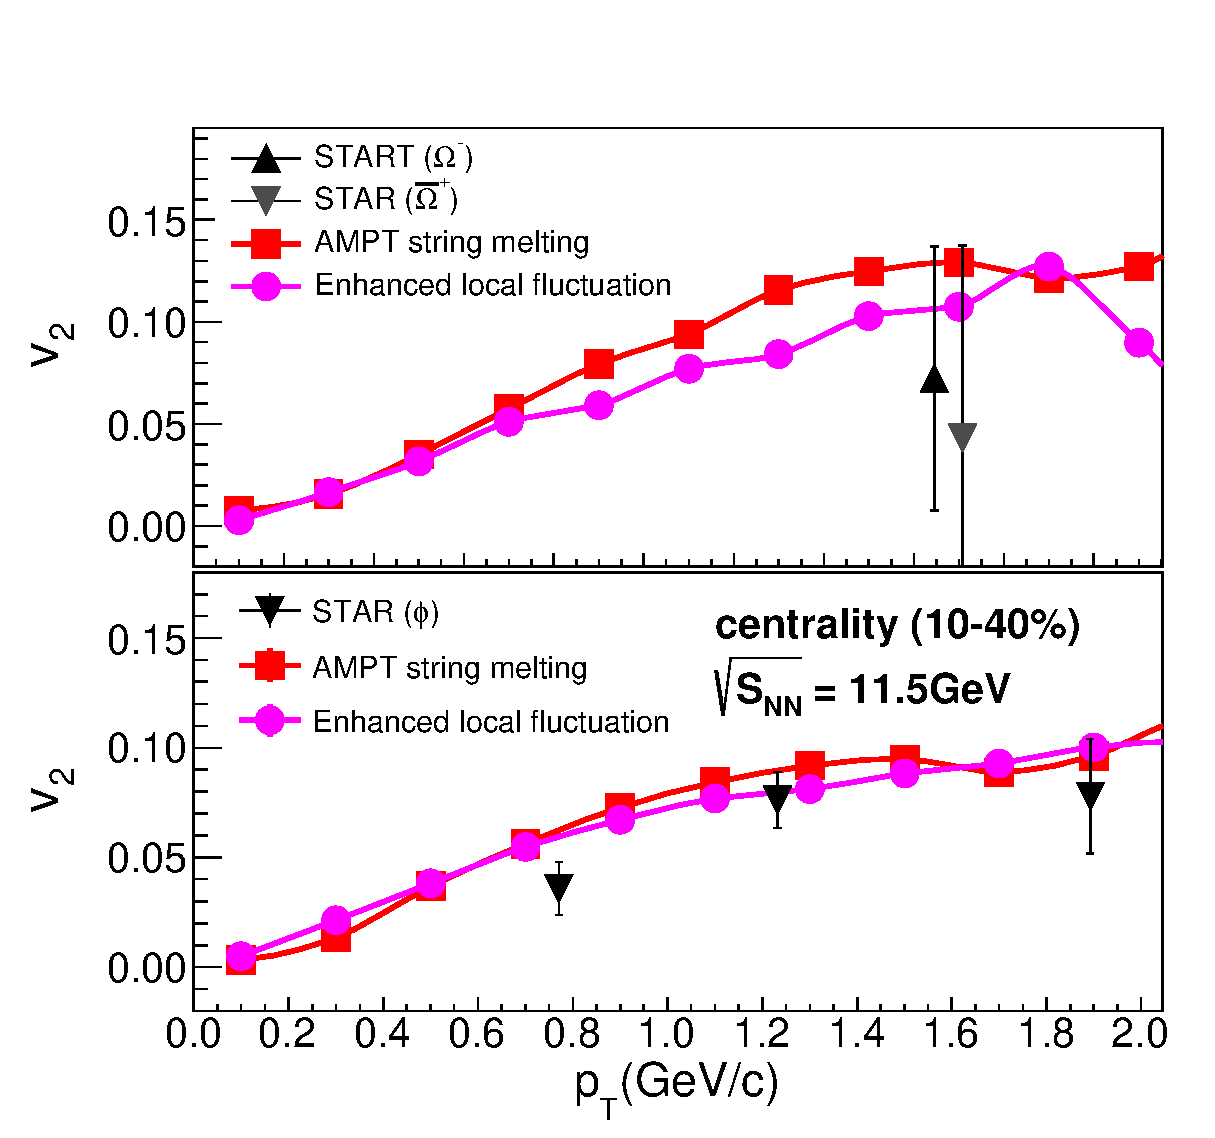
\includegraphics[width=0.45\textwidth]{./figure/flow.eps}
  \caption{The elliptic flow: upper panel is $\Omega$ flow, bottom panel is $\phi$ flow.}
  \label{fig:figureflow}
\end{figure}
In Fig. \ref{fig:figureflow}, we show the results of $v_{2}$. In  the range of experiment error, the data from string melting AMPT and
enhanced local fluctuation AMPT can be consistent with the experiment. Comparing the
two sets of AMPT model data, the size of  $v_{2}$ is almost same. because, In AMPT
model, the $v_{2}$ is mainly developed in the parton cascade stage, moreover,
the $v_{2}$ of $\Omega$ and $\phi$ is not affected by the hadron interaction due to its
small cross-section.

\section{Summary}
Based on the parton phase-space information and dynamical coalescence method, we study the effect
of QCD fluctuation on the production of $\Omega$ baryon and $\phi$ meson. we have calculated the
transverse momentum spectra, ratio and elliptic flow of these particles. For the production of
$\Omega$ and $\phi$, we have found that the QCD fluctuation have the trend to increase the ratio
of baryon-to-meson, it can be used as a valid evidence for detecting the QCD critical point.
For the $v_{2}$ of $\Omega$ and $\phi$, we have found that it is not sensitive to the QCD
fluctuation.















\begin{thebibliography}{88}
\bibitem{AMPT1} B. Zhang, C. M. Ko, B. A. Li, and Z. W. Lin, Phys. Rev. C
  \textbf{61}, 067901 (2000).

\bibitem{AMPT2} Z. W. Lin, S. Pal, C. M. Ko, B. A. Li, and B. Zhang, Phys. Rev. C
  \textbf{64}, 011902 (2001).

\bibitem{AMPT3} Z. W. Lin, C. M. Ko, B. A. Li, B. Zhang and S. Pal, Phys. Rev. C
  \textbf{72}, 064901 (2005).

\bibitem{AMPT4} B. Zhang, C. M. Ko, B. A. Li, Z. W. Lin, and B. H. Sa, Phys. Rev. C
  \textbf{62}, 054905 (2000).

\bibitem{FLOW1} Y. C. He and Z. W. Lin, arXiv:1703.02673v1 [nucl-th]

\bibitem{HIJING1} X. N. Wang, Phys. Rev. D
  \textbf{43}, 104 (1991)

\bibitem{HIJING2} X. N. Wang, and M. Gyulassy, Phys. Rev. D
  \textbf{44}, 3501 (1991)

\bibitem{ZPC} B. Zhang, Comput. Phys. Commun.
  \textbf{109}, 193 (1998)

\bibitem{ART1} B. A. Li and C. M. Ko, Phys. Rev. C
  \textbf{52}, 2037 (1995).

\bibitem{ART2} B. A. Li, A. T. Sustich, B. Zhang, and C. M. Ko, Int. J. Mod. Phys. E
  \textbf{10}, 267 (2001).

\bibitem{CROSSSECTION} Z. W. Lin and C. M. Ko, Phys. Rev. C
  \textbf{65}, 034904 (2002).

\bibitem{TENMB} L. W. Chen and C. M. Ko, Phys. Rev. C
  \textbf{73}, 044903 (2006).

\bibitem{COALESCENCE1} R. Mattiello, A. Jahns, H. Sorge, H. Stocker and W. Greiner
  Phys. Rev. Lett. \textbf{74}, 2180 (1995).

\bibitem{COALESCENCE2} L. W. Chen, C. M. Ko and B. A. Li, Phys. Rev. C
  \textbf{68}, 017601, (2003).

\bibitem{SONGTEACHER} S. Zhang, J. H. Chen, H. Crawford, D. Keane, Y. G. Ma and Z. B. Xu
  Phys. Lett. \textbf{B684}, 224 (2010).

\bibitem{STAR} L. Adamczyk el al. (STAR Collaboration), Phys. Rev. C
  \textbf{93}, 021903(R) (2016).

\bibitem{MALONG} L. Ma, G. L. Ma and Y. G. Ma, Phys. Rev. C
  \textbf{89}, 044907 (2014).
\end{thebibliography}
\end{CJK*}

\end{document}

%%% Local Variables:
%%% mode: latex
%%% TeX-master: "refercence"
%%% End: